\chapter{Cyber Realm of War in Ukraine}

The conflict in Ukraine had a significant impact on international relations. This study seeks to examine the patterns and trends observed in the cyber aspect of the Ukrainian conflict, specifically focusing on the defining characteristics of the cyber realm within this context. Furthermore, it aims to evaluate the strategic efficacy of the cyber operations employed during the war between Ukraine and Russia.  By leveraging these resources, this research aims to offer a comprehensive analysis of the cyber dimension of the Ukrainian conflict, fostering a deeper understanding of its implications. This chapter critically examines the failure of Russian cyber operations in Ukraine by analysing significant cyber events that occurred during wartime, assessing the accountability of Russian cyber troops, and evaluating the extent of Western assistance. The outcome of this analysis will show the main characteristics of cyber operations in wartime, which will be searched on the European cyber strategies further in this work.

The hypothesis behind this study rests on the Russian failure in its cyber operations in Ukraine, not only due to the Western assistance, which has been widely discussed in the literature but also because of the inefficiency in the preparation and execution of military and cybernetic plans. While we have evidence of the kinetic side failure, the same cannot be said for cyberspace. In this regard, the work aims to develop further this topic.

The cyber dimension of the war in Ukraine has garnered significant attention and interest among researchers and analysts. Numerous studies have delved into the intricate patterns and evolving trends of cyber-attacks, assessing the strategic effectiveness of cyber operations, and contemplating broader implications for future conflicts. Companies directly involved, such as Microsoft and Google, have progressively developed analyses of Ukrainian cyberspace, presenting the main Russian cyber operations and how they support cyber defence.

Additionally, the research work will employ insightful research from the Carnegie Endowment for International Peace collection on cyber conflict in the Russia-Ukraine War. These studies explore cyber events chronologically, providing strategic significance \parencite{levite_2023_integrating, lewis_2022_cyber}, while others focus on the structural problems of inter-institutional cooperation within the Russian agency regarding cyber operations \autocite{wilde_2022_cyber}. The literature agrees with defining the war outcomes, both from the cyber and kinetic perspectives, as a failure of the Russian Federation. However, there were differences in the key factors that led to this outcome.

According to \textcite{lin_2022_russian}, Russian cyber failure relies on the unpredictability of cyber operations, which has caused Russian military command to avoid their strategic use, instead of relying on hard military power. Moreover, scholars agree that Western assistance has strongly influenced Ukraine's cyber defence in various ways. \textcite{beecroft_2022_evaluating} qualitatively analysed how the West helped Ukraine build a more resilient defence.

Finally, this chapter will rely on CyberPeace Institute Quarterly research, a highly reputable NGO specializing in cyber politics, to avoid political bias that may be present in such a theme. The latter provides us with the opportunity to explore data on cyber operations from both sides of the conflict, with a focus on human rights.

\section{Exploring the Cyber Dimension of the Russian Invasion of Ukraine}

On February 24, 2022, the events had a profound and lasting impact on international relations. The visual portrayal of bombings in Ukrainian cities served as a stark reminder, while the consequential political and economic effects reverberated globally. Simultaneously, as Russian Main Battle Tanks (MBTs) and Armoured Personnel Carriers (APCs) breached the Ukrainian border, the cyber domain played an integral role in both laying the groundwork and disrupting the adversary. Despite facing a significantly more powerful opponent in the Russian military, Ukraine showed remarkable resilience, not only withstanding the onslaught but also mounting counteroffensives that decisively shifted the balance of power on the battlefield.

\subsection{Overview between Russian cyberattackers and Ukraine cyberdefenders}
Before starting our discussion, it is crucial to identify the relationship between Russian cyber and kinetic forces, especially by emphasising the inter-institutional relationships between different realities. Comparing them to the Ukraine counterpart is also beneficial to the discussion, to have an overview of forces that were (and are) in the cyber field.  

\textbf{Russia Cyber Structure}

The first main difference between Western and Russian cyber-attitudes relies on the term used to identify those actions in the cybernetic environment. Russians do not use the term cyber; instead, they refer to the information (\textit{informatsiya}) confrontation in the political and military lexicon to describe the range of operations—both technical and psychological, code, and content—that can be deployed against adversarial systems and decision-making \autocite[3]{wilde_2022_cyber}. This perspective is prevalent in Russia, and can be traced back to the Soviet era. It significantly influences not only the methodologies employed by Russia, but also the objectives pursued through its global-scale information operations. Offensive cyber operations constitute a specific subset of operations that seek to influence the information environment. These are integral components of a broader spectrum of operations that share the common objective of influencing the environment. For the purposes of our research, we adopt the term cyber to encompass all operations aimed at exerting influence on the information environment through the use of computer networks and electronic systems.

\begin{figure}[H]
\centering
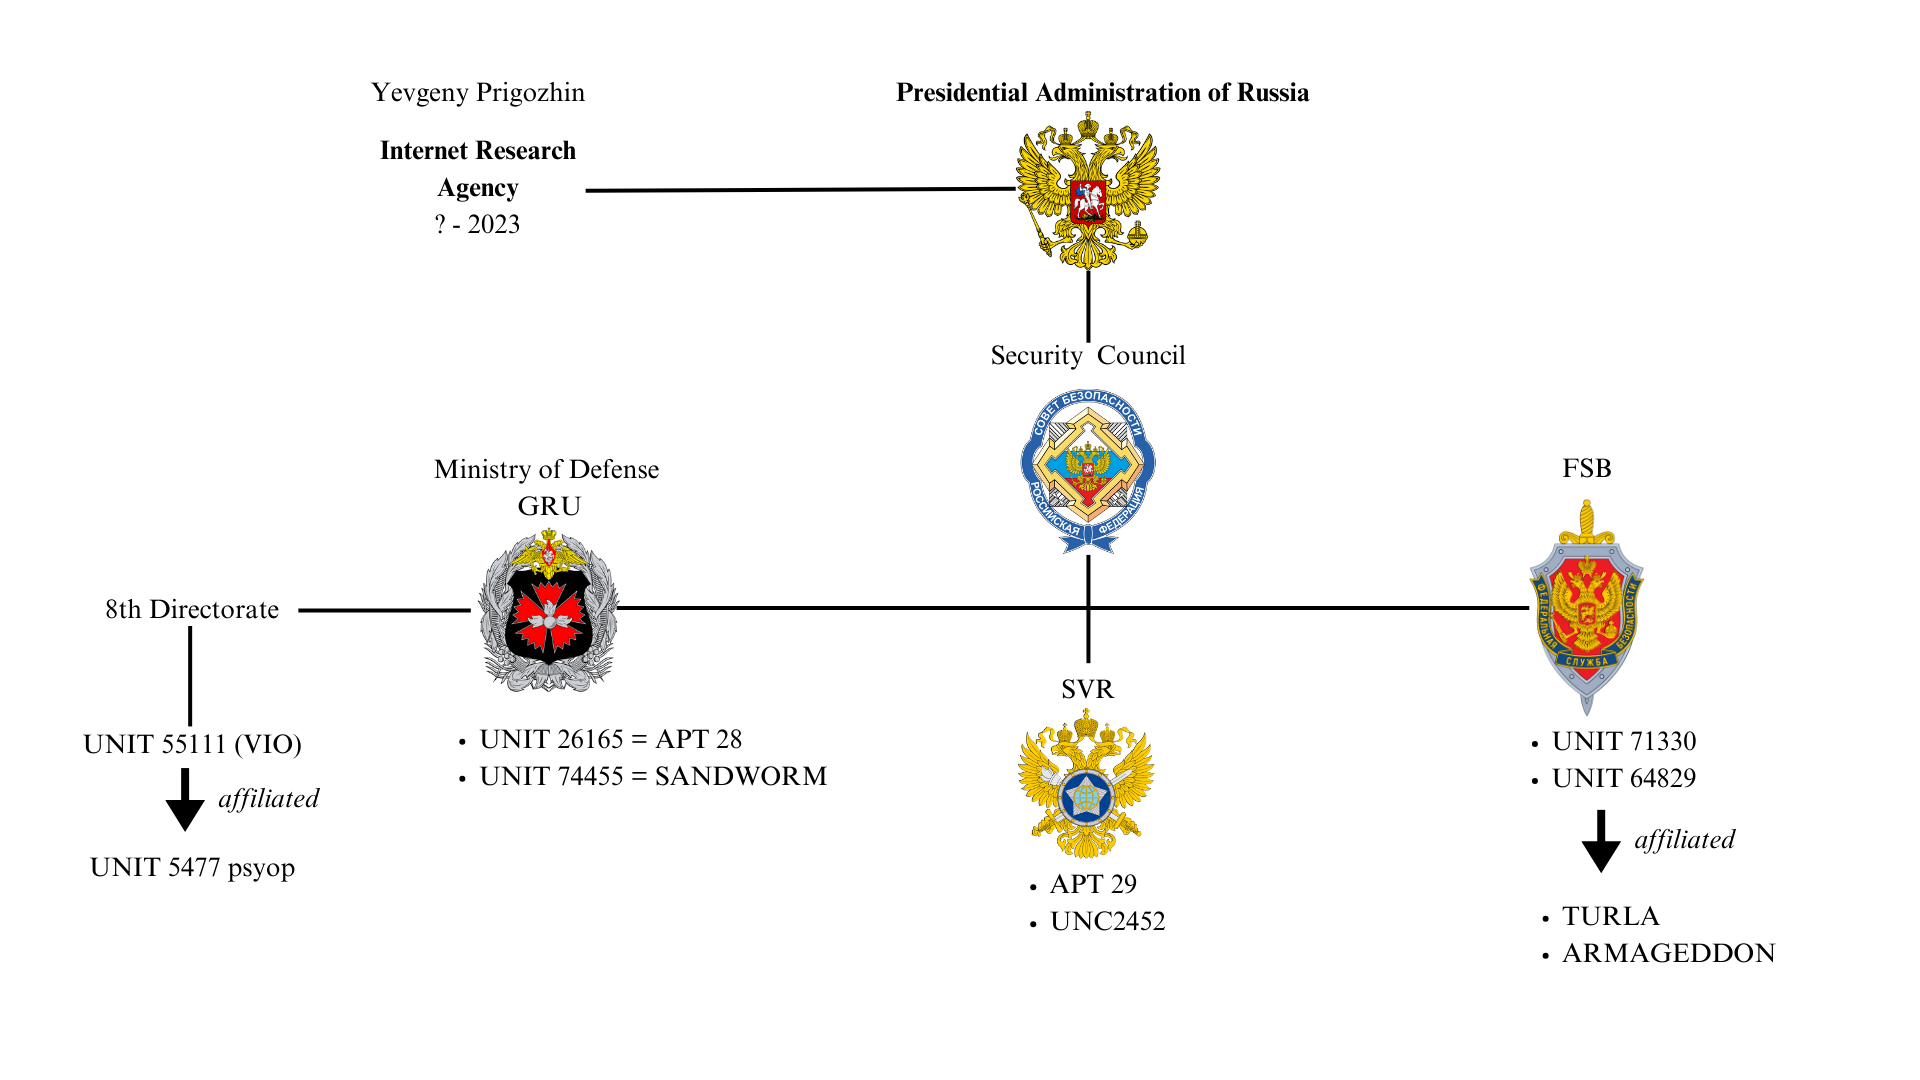
\includegraphics[width=1\textwidth]{Images/RussiaCyber.png}
\caption{\textit{Russia Cyber Structure. Author's representation from \textcite{wilde_2022_cyber} and Mandiant}}
\label{RussiaCyber.png}
\end{figure}

Historically, the information environment was under the exclusive control of security agencies in the Soviet Union, such as the KGB. As a result, modern Russian bureaucracy continues to adhere to the principles established by Soviet \textit{nomenklatura}, even in the realm of cyber operations. In recent times, Western intelligence communities, in cooperation with threat intelligence companies such as Mandiant and Recorded Future have tried to link Russian threat actors with their bureau, in order to understand their task as state-sponsored threat actors. 

Most Russian operations are conducted by \textit{Glavnoye Razvedyvatelnoye Upravlenie} (GRU), the foreign military intelligence agency of the Russian Federation, specifically through Unit 54777. This unit is part of a larger institutional organization known as \textit{Voyska Informatsionnykh Operatsiy} (VIO), or Information Operations Troops. The actions of the Russian cyber apparatus are directly supervised and guided by the Security Council, exemplifying political control over military mechanisms \autocite{wilde_2022_cyber}. The literature offers numerous examples of how Unit 54777 operated during peacetime, exerting influence over political scenarios (e.g., Georgia 2008), disrupting critical services (e.g., Estonia 2007), and attempting to influence electoral processes (e.g., United States 2016). Unit 54777 specialised in psychological operations, considered the feature with the most impact on the Russian cyber strategy \autocite{wilde_2022_cyber}.

Official cyber units that are embedded with the Russian military organisation are hardly recognised for their methods of attack. For this reason, threat intelligence services categorise Russian threat actors with code-names to simplify the clustering, while attempting to link with the Russian military structure. For instance, the Foreign Intelligence Service known as SVR (\textit{Služba Vnešnej Razvedki}) have several groups affiliated, as the APT29 is often mentioned as \textit{Cozy Bear} or the GRU Unit 745455 mentioned as \textit{Sandworm}. Mentioning the names and code-names of Russian cyber units and threat actors is important for several reasons, ranging from technical attribution to political implications. Technical attribution is established by comprehending the tactics, techniques, and procedures (TTPs) employed in cyberattacks. On the other hand, the political response involves public condemnation and establishing the link between the threat actor and their affiliated unit, often leading to sanctions imposed by the victim.

\textbf{Ukraine Cyber Structure}

Ukraine's cyber-structure has been less researched than its Russian counterpart, for obvious reasons. Since the Donbas crisis and the Russian annexation of Crimea in 2014, Ukraine has been constantly under target by Russian-led cyber operations. In 2016, Ukraine approved its first cybersecurity strategy, which acknowledged that the country's cyber infrastructure had been attacked and emphasised the need for a formal cybersecurity system. This system was designed to counter cyberterrorism and protect critical infrastructures, including the military, energy, transportation, and banking sectors. The strategy also proposed that the state would work with NATO and EU members to establish best practices \autocite{brantly_2019_cybersecurity}.

The structure of cybersecurity in Ukraine is primarily centralised and falls under the National Security and Defence Council (NSDC). The NSDC encompasses the Ministry of Defence (MoD), the Security Service of Ukraine (SBU), Ministry of Internal Affairs (MIA), the Main Directorate of Intelligence, and the State Service of Special Communications and Information Protection of Ukraine (SSSCIP). The structure, as will be discussed in the following sections, as been relatively proactive in cooperating with other intelligence agencies and private companies that have offered their know-how to support Ukraine's defence against Russian invasion. 

After the Russian invasion, the Ministry for Digitalization called for the establishment of the IT Army of Ukraine, in which every person has the possibility to contribute to disruptive attacks (such as DDoS) from their own device and network on specific targets (like Russian websites and networks). It was the first time that a government called for collective action against cyberattacks, simplifying the methods \footnote{By joining a telegram channel and downloading the script, the user could start the attack with one click.} with the aim of collecting fire powers for their objectives. 

\begin{figure}[H]
\centering
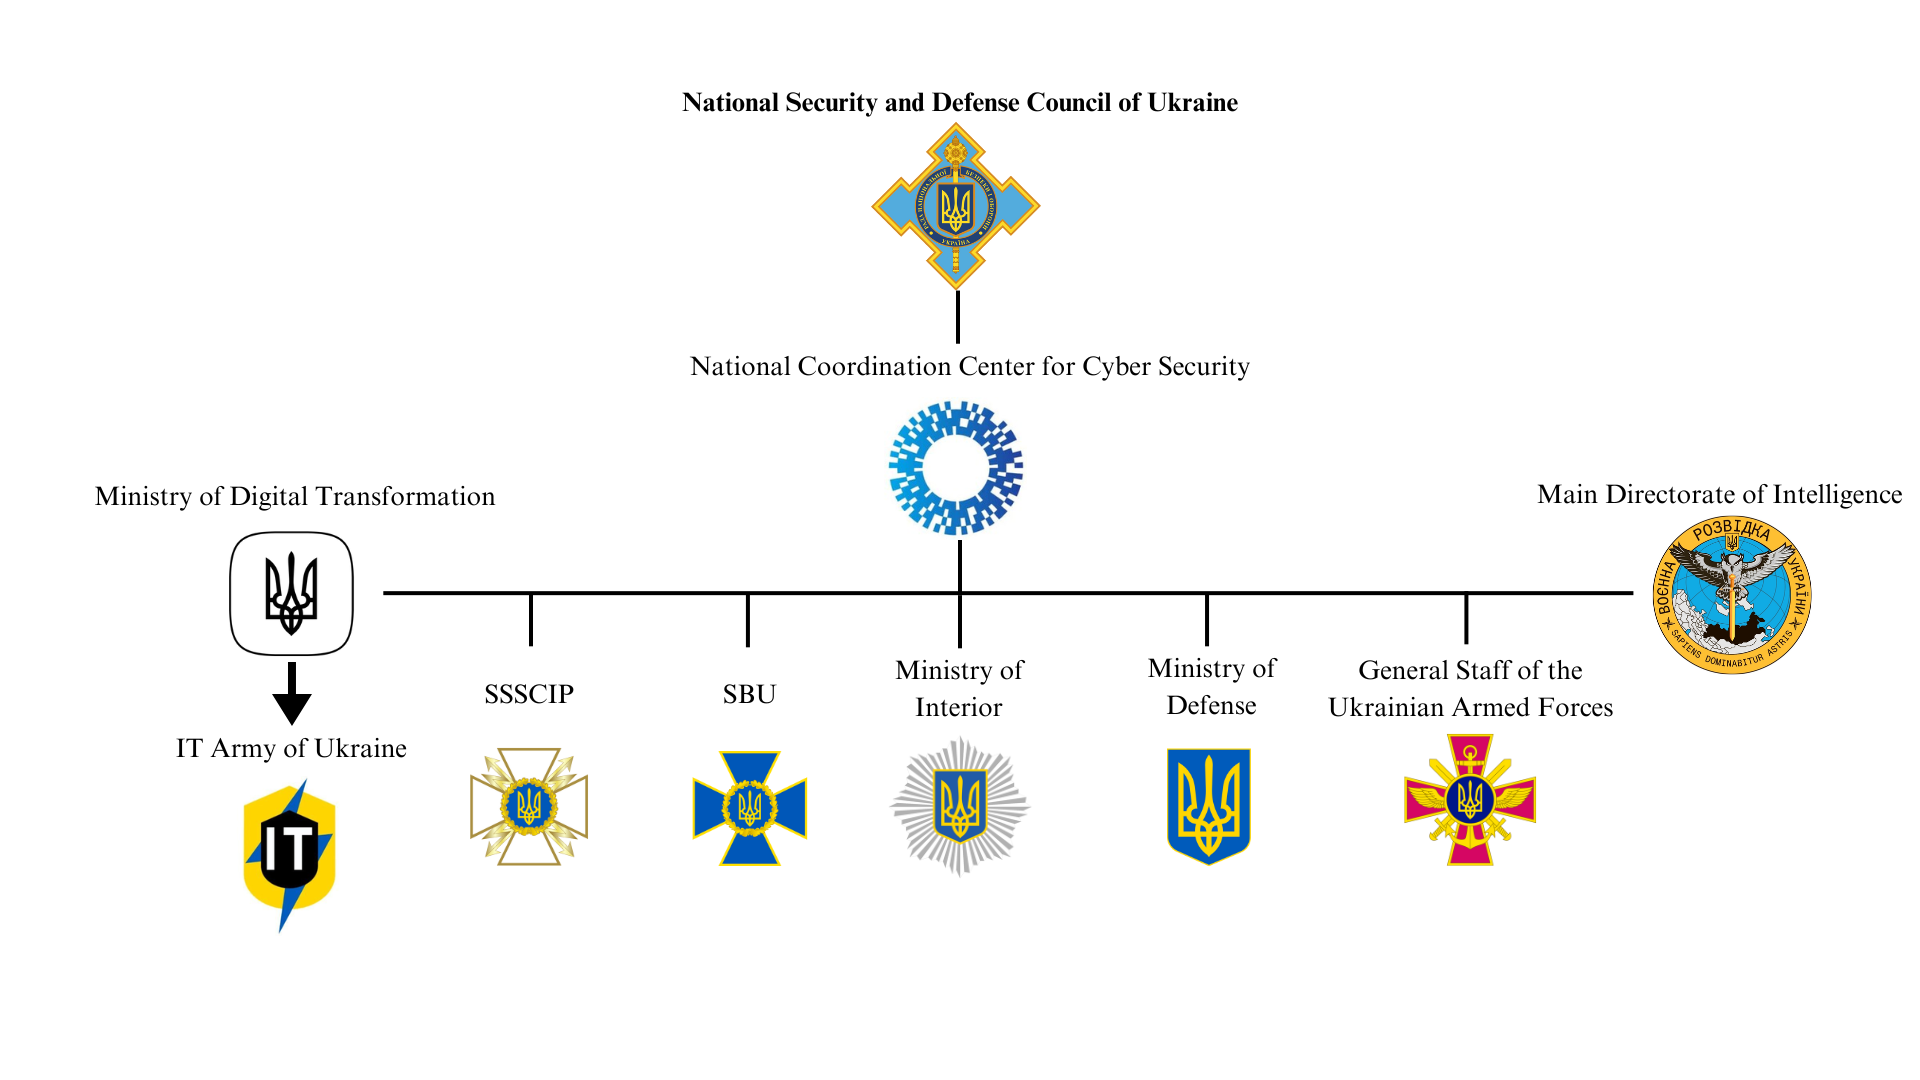
\includegraphics[width=1\textwidth]{Images/UkraineCyber.png}
\caption{\textit{Ukraine Cyber Structure. Author's representation from \textcite{brantly_2019_cybersecurity}}}
\label{UkraineCyber.png}
\end{figure}

\section{Examples of Russian Cyber Operations in Ukraine}

Tensions between Russia and Ukraine emerged prior to the 24th of February, manifested through the Crimean annexation and the Donbas conflict. Even after more than a year of fighting, the Russian Federation was unable to succeed in toppling the Kyiv government. This protracted conflict exposed the military challenges and setbacks faced by Russian forces, reminiscent of their experiences in the Chechen wars. Similarly, the outcomes of cyber operations mirrored those of kinetic military actions. Russian cyber offensives, as documented by \textcite{baetman_2022_russias}, did not yield a significant strategic impact on the overall course of the war.

On the day preceding the outbreak of the war, Russia conducted a disabling attack on Viasat's European satellite network. This targeted assault resulted in the disruption of Internet services for numerous Viasat customers in Ukraine, leading to communication breakdowns across various government agencies and businesses \autocite{willett_2022_the}. This attack stands out as a significant accomplishment of Russian forces in the realm of cyberspace. Dmitri Alperovitch\footnote{ Dmitri Mikhailovich Alperovitch is an American think-tank founder, investor, philanthropist, podcast host and former computer security industry executive.} referred to it as the most strategically impactful cyber operation in the history of wartime \autocite{baetman_2022_russias}. However, achieving effective coordination between cyberweapons and kinetic weapons poses considerable challenges. The limited strategic impact of the cyber dimension compared to its kinetic counterpart can be attributed to the integration of both domains within a combined arms approach \autocite{wilde_2022_cyber}. The Russian Voyska Informatsionnykh Operatsiy (VIO) lacked prior experience and empirical preparation for conducting destructive cyber operations during wartime. Bureaucratic obstacles have hindered efficient cooperation between agencies and the military, impeding their effectiveness in the cyber domain.

Military operations in Ukraine underwent significant changes compared to the initial expectations of a swift campaign aimed at overthrowing the Kyiv government, similar to the annexation of Crimea in 2014. However, due to Ukraine's exceptional defence capabilities and support from Western nations, the war's outcome shifted, transforming it into a war of attrition. In this attrition-based conflict, offensive cyber operations proved less suitable. The nature of cyber-attacks requires meticulous preparation and intelligence gathering, which cannot keep up with the fast-paced nature of kinetic military operations during wartime \autocite{beecroft_2022_evaluating}.

Notably, these difficulties have been empirically verified through an analysis of cyber targeting in Ukraine. Russia has predominantly utilised cyber firepower to target Ukraine's critical infrastructure. During the initial weeks of the war, Russia employed Industroyer2 malware to target the management system of the electricity grid, although no power outages occurred \textcite{willett_2022_the}. Between January 2022 and March 2023, the CyberPeace Institute documented 360 cyber incidents targeting entities in Ukraine \autocite[3a]{cyberpeaceinstitute_2023_cyber}. Microsoft, a significant contributor to Ukraine's cyber defence, stated that most destructive cyberattacks had been successfully repelled, resulting in no critical disruptions for either civilian or military sectors, except for the Viasat hack \autocite{smith_2022_defending}. However, a potential correlation between cyberattacks and kinetic attacks is worth noting. On March 4, a GRU-affiliated cyber group targeted the Vinnystia government network, followed by cruise missile strikes on March 6 and 16, targeting the Vinnystia airport and TV tower, respectively \autocite[8]{smith_2022_defending}. According to Bateman, these cyberattacks do not seem to cause any disabling effects, rendering them unsuccessful. If they were coordinated with physical attacks, they either failed to achieve the intended effects or were conducted as cyber intelligence operations in support of kinetic targeting \autocite[9]{baetman_2022_russias}. It is plausible to hypothesise that kinetic operations in Ukraine were deployed as an independent instrument aimed at tactical objectives, rather than serving as a complementary strategy to cyber operations. Another example of the cyber-kinetic paradigm can be observed on March 1, when the Russian military publicly declared its intention to destroy information-based targets in Ukraine, followed shortly by a missile strike on a TV tower in Kyiv. It is noteworthy that prior to this incident, Microsoft alerted Ukrainian authorities about a failed destructive cyberattack targeting a prominent broadcasting company \parencite{baetman_2022_russias, smith_2022_defending}. Microsoft stated that computer network operators and physical forces independently pursued a common set of priorities \autocite{microsoft_2022_an}. 

One successful attempt was related to the Sandworm attack on Ukraine's power grid which causes a power blackout before a missile attack in late 2022 \footnote{Mandiant (Google) have release a report on it: https://www.mandiant.com/resources/blog/sandworm-disrupts-power-ukraine-operational-technology}. This type of attack represent an evolution in the cyber-kinetic integration on the Russian side, suggesting that their experience were useful to improve their capabilities. 

Although assessing the effectiveness of integrated cyber-kinetic attacks is challenging, some scholars have attempted to analyse them through case studies and assess their tactical, operational, and strategic outcomes. For example, Bateman analysed the Dnipro cyber and kinetic attacks on March 11. Although the Russian forces achieved permanent deletion of government agency data at the tactical level, the delay in emergency response to missile strikes had only marginal operational benefits. Furthermore, the strategic objective of a ground assault is neither achievable nor attempted \autocite[11]{baetman_2022_russias}.



The literature has produced several details because Russian cyber fires did not have a strategic role in the Ukraine War. Building upon the prevailing scholarly perspectives, this study contributes an additional explanation to further explore this phenomenon.

\section{Intelligence gathering rather than destruction}

Scholars concur that Russian cyber assets are primarily employed for intelligence gathering \parencite{baetman_2022_russias, levite_2023_integrating, beecroft_2022_evaluating, lin_2022_russian}. Assessing the pre-war cyber intelligence gathering activities of Russia presents inherent challenges; nevertheless, it can be argued that the strategic failure of the special military operation was significantly impacted by Russian agencies' underestimation of Ukraine's political and military capabilities. Moreover, criticism has been directed towards Russian intelligence agencies for their unreliable human sources within Ukraine, instances of financial misappropriation, historical deficiencies in analytic proficiency, and pervasive inter-service rivalries, all of which have contributed to a compromised operational environment \autocite{baetman_2022_russias}. There could be two hypotheses as to why cyberintelligence gathering was preferred over destructive gathering. First, Russian cyber forces are trained to operate during peacetime, favouring intelligence gathering over the destruction of information. As assessed previously for infrastructure targeting, it is possible that kinetic instruments were used when destructive cyber operations failed, preferring to use intelligence to better calibrate kinetic actions. However, this does not exclude the capacity of Russian forces to execute destructive cyber-attacks, as seen in NotPetya. Scholars such as \textcite{lin_2022_russian} and \textcite{levite_2023_integrating} affirmed that Russia was restrained in using its top-tier cyber assets to avoid spillover and retaliation from Western countries. They also believe that Russia may be maintaining its full cyber capacity under the shadows for future confrontations with NATO. These theses could be misleading because Russia has used its best kinetic military assets in Ukraine and showed their fallibility (several exemplars of T-90 destroyed, Kinzhal supersonic missiles intercepted, BMPT Terminator destroyed\footnote{Full list of Russian losses documented with video and photo can be found on the Oryxs website: https://www.oryxspioenkop.com/2022/02/attack-on-europe-documenting-equipment.html}).

Achieving a Cyber Pearl Harbor during wartime is not just a matter of coordination with the kinetic side, but rather a complex issue that relates to assets that are far away from being ready. For instance, during the DEFCON 2015 \textcite{krotofil_2015_rocking} presented a case study on attacking a chemical plant. The lesson learned was that achieving kinetic destruction or disruption of critical infrastructure such as a chemical plant is less intuitive than expected. The attacker should have high knowledge of chemicals, be able to reproduce the attack in the laboratory (as the Stuxnet perpetrator did), to be able to overcome changes in different chemical plants that are connected to each other. The plan becomes expensive and too risky to be executed. However, if the attack succeeds, the complexity will play against the defender as well \autocite{drozhzhin_2015_hacking}. This short case study gives us the opportunity to better understand what the priority is for countries and regional organizations that are building up a coherent cyber defence strategy. Strengthening Critical Infrastructure protection is fundamental, however, decision-makers need to put efforts into understanding that no cyber Pearl Harbor will happen in the near future and less destructive cyber operations such as cyber espionage are a big issue in the long term that affects both the military and civil side of cyberspace. 

\section{Western Assistance}

One of the main reasons for the efficiency of Ukraine's cyber defence lies in Western support. Western countries, primarily NATO members, provided Ukraine with air defence systems and MTBs, as well as support in the cyberspace domain. In this regard, it is important to distinguish between the contributions of private companies and the government. One Ukrainian cyber defender was Microsoft, which invested \$239 million without charge to aid Ukraine's cyber defence \autocite{smith_2022_defending}. Microsoft has contributed to the migration of government data to cloud servers located far from the conflict zone, specifically in the Baltics and Poland. Microsoft actively disrupted Russian cyber operations, conducted cyber threat intelligence, ensured business continuity for the private sector in Ukraine, and secured government cyber assets. However, Google, along with its Cyber Threat branch Mandiant, disrupted 1,950 Russian influence operations in 2022 aimed at spreading fake news and discrediting Western assistance in Ukraine. Google developed the Rapid Air Missiles Alert for Android smartphones, which informed civilians about upcoming Russian missile attacks \autocite{huntley_2023_fog}. Other private actors, such as Cisco, Cloudflare, and Amazon, also contributed to various aspects of Ukraine's cyber defence \autocite{beecroft_2022_evaluating}. Special mention should be made to SpaceX, which provides telecommunications services with its Starlink after the cyberattack on Viasat.

From a governmental perspective, the main contributors were the UK Foreign, Commonwealth, and Development Office (FCDO) and the UK National Cyber Security Centre (Champion, as cited in Beecroft, 2022). Additionally, the U.S. The Cyber Command and the EU Cyber Rapid Response Teams deployed cybersecurity personnel prior to the invasion to defend Ukraine's networks \autocite[3]{beecroft_2022_evaluating}. It is important to note that all the private and governmental actions taken to enhance Ukraine's cyber resilience were not centrally orchestrated according to a unified plan, but rather constituted an agglomeration of activities driven by various stakeholders. The Ukrainian National Cybersecurity Coordination Center, established in 2016, played a key role in synchronizing these disparate operations and actors \autocite[3]{beecroft_2022_evaluating}.

Nevertheless, Ukraine has significantly bolstered its cyber defence capabilities following the \textit{NotPetya} attack and gained valuable experience in countering Russian cyber operations. In fact, as of May 2023, Ukraine officially joined the NATO Cooperative Cyber Defence Center of Excellence (CCDCOE), offering a unique opportunity to both contribute to Ukraine's defence in Russia's brutal war and learn from the cyber battlefield to enhance the cybersecurity of all members. This war underscored the pivotal role of private tech companies during wartime as game changers capable of influencing conflict outcomes. Microsoft President and Chairman Brad Smith emphasised the necessity of a collective cyber defence organisation for a coordinated and comprehensive strategy to strengthen cyber defence \parencite{smith_2022_defending, beecroft_2022_evaluating}.

\section{The role of Hacktivists during wartime}

The disruptions through DDoS attacks have increased significantly after the Russian invasion of Ukraine. Russian hacktivists have targeted mainly European partners of Ukraine as an act of retaliation for their military and diplomatic support. One of the most active cyber actors are NoName057(16), a collective cyber militia which is fighting for the Russian cause in cyberspace. Since April 2023, NoName057 have conducted more than 2,500 attack operations  Those hacktivists have disrupted major financial, transport and government websites even more than one time in a row.  Remarkable the case of the Italian websites of Carabinieri and Ministry of Labour, attacked the fifth time in a row, underlining the incapacity of Italian authorities to react and counter the attack \autocite{redhotcyber_2023_colpito}. This example is a prelude that European countries and their private companies are not able to guarantee most of the time the security of their IT infrastructure. The disruptions through DDoS attacks have increased significantly after the Russian invasion of Ukraine. Russian hacktivists have targeted mainly European partners of Ukraine as an act of retaliation for their military and diplomatic support. 

Another hacktivist group that has targeted Ukraine and Western countries are KillNet. Killnet is a collective of hacktivists, such as Anonymous Sudan, REvil and Anonymous Russia, among others. While no proof has been found for the connection with the Russian government, Mandiant believes that coordination with Russian authorities is plausible \autocite{mandiant_2023_killnet}. As with all hacktivist groups, the ideology is the core of their activity. In this case, the geopolitical strategy of Russia is clearly present in KillNet’s operations. Notably, KillNet capabilities are constantly increasing \autocite{mandiant_2023_killnet}, offering the power to attack even secured networks of NATO and National defence agencies. KillNet represents a threat that Western countries could not underestimate and counter not only from a technical perspective but also from a political discourse. 

\begin{figure}[H]
\centering
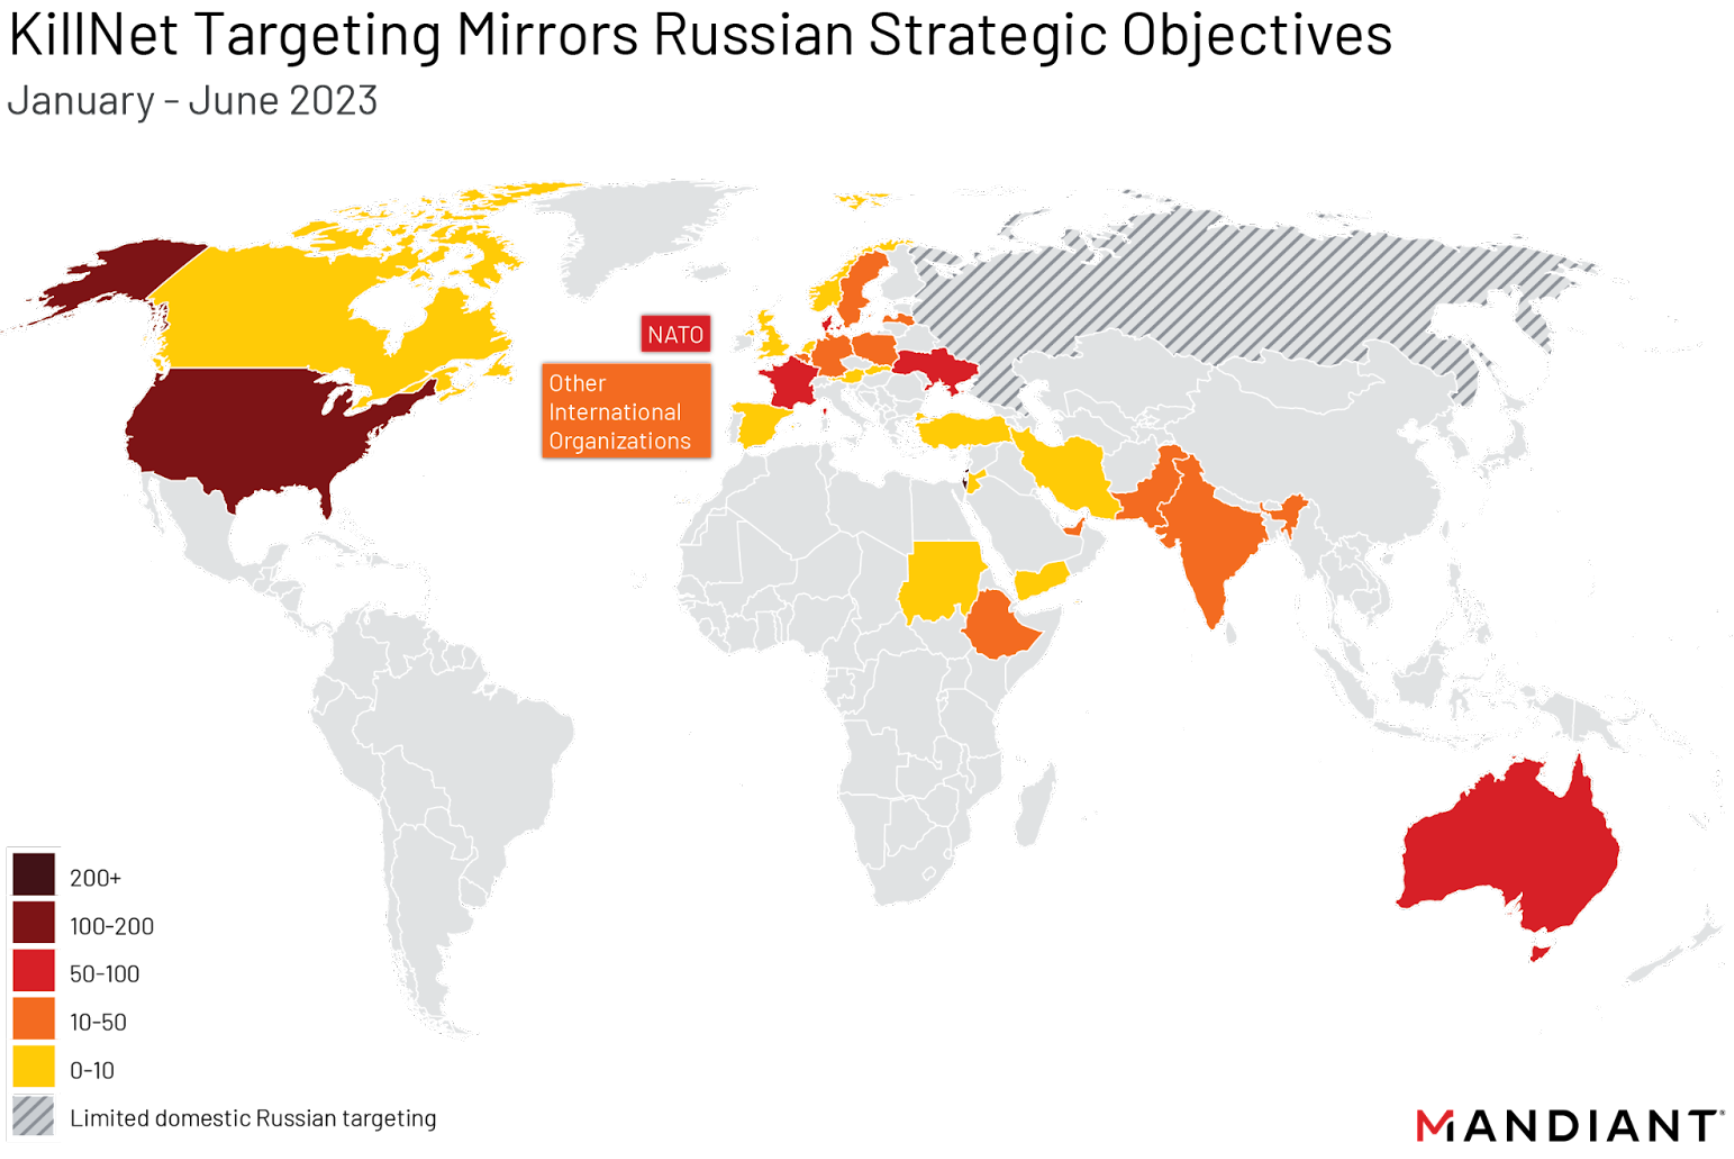
\includegraphics[width=0.8\textwidth]{Images/killnet.png}
\caption{\textit{Killnet attacks overview by \textcite{mandiant_2023_killnet}}}
\label{killnet.png}
\end{figure}

From the Ukrainian side, Anonymous and Anonymous Italia have been the primary actors in the field, excluding the government-affiliated IT Army of Ukraine. One of their objectives was to disrupt government websites and telecommunications. Remarkable action was the hack of several Russian televisions to show Russian citizens an independent coverage of the war in Ukraine\footnote{For more information: https://www.rferl.org/a/russian-tv-hacked-ukraine-anonymous/31740663.html}, since almost all the media are not allowed to diverge from the government perspective. 

Since February 2022, the threat actors number has increased constantly. As minefields or unexploded that would be difficult to find and disarm before some other incident after war, also the hacktivists will not cease to be active and other \textit{missions} will be found. 

\begin{figure}[H]
\centering
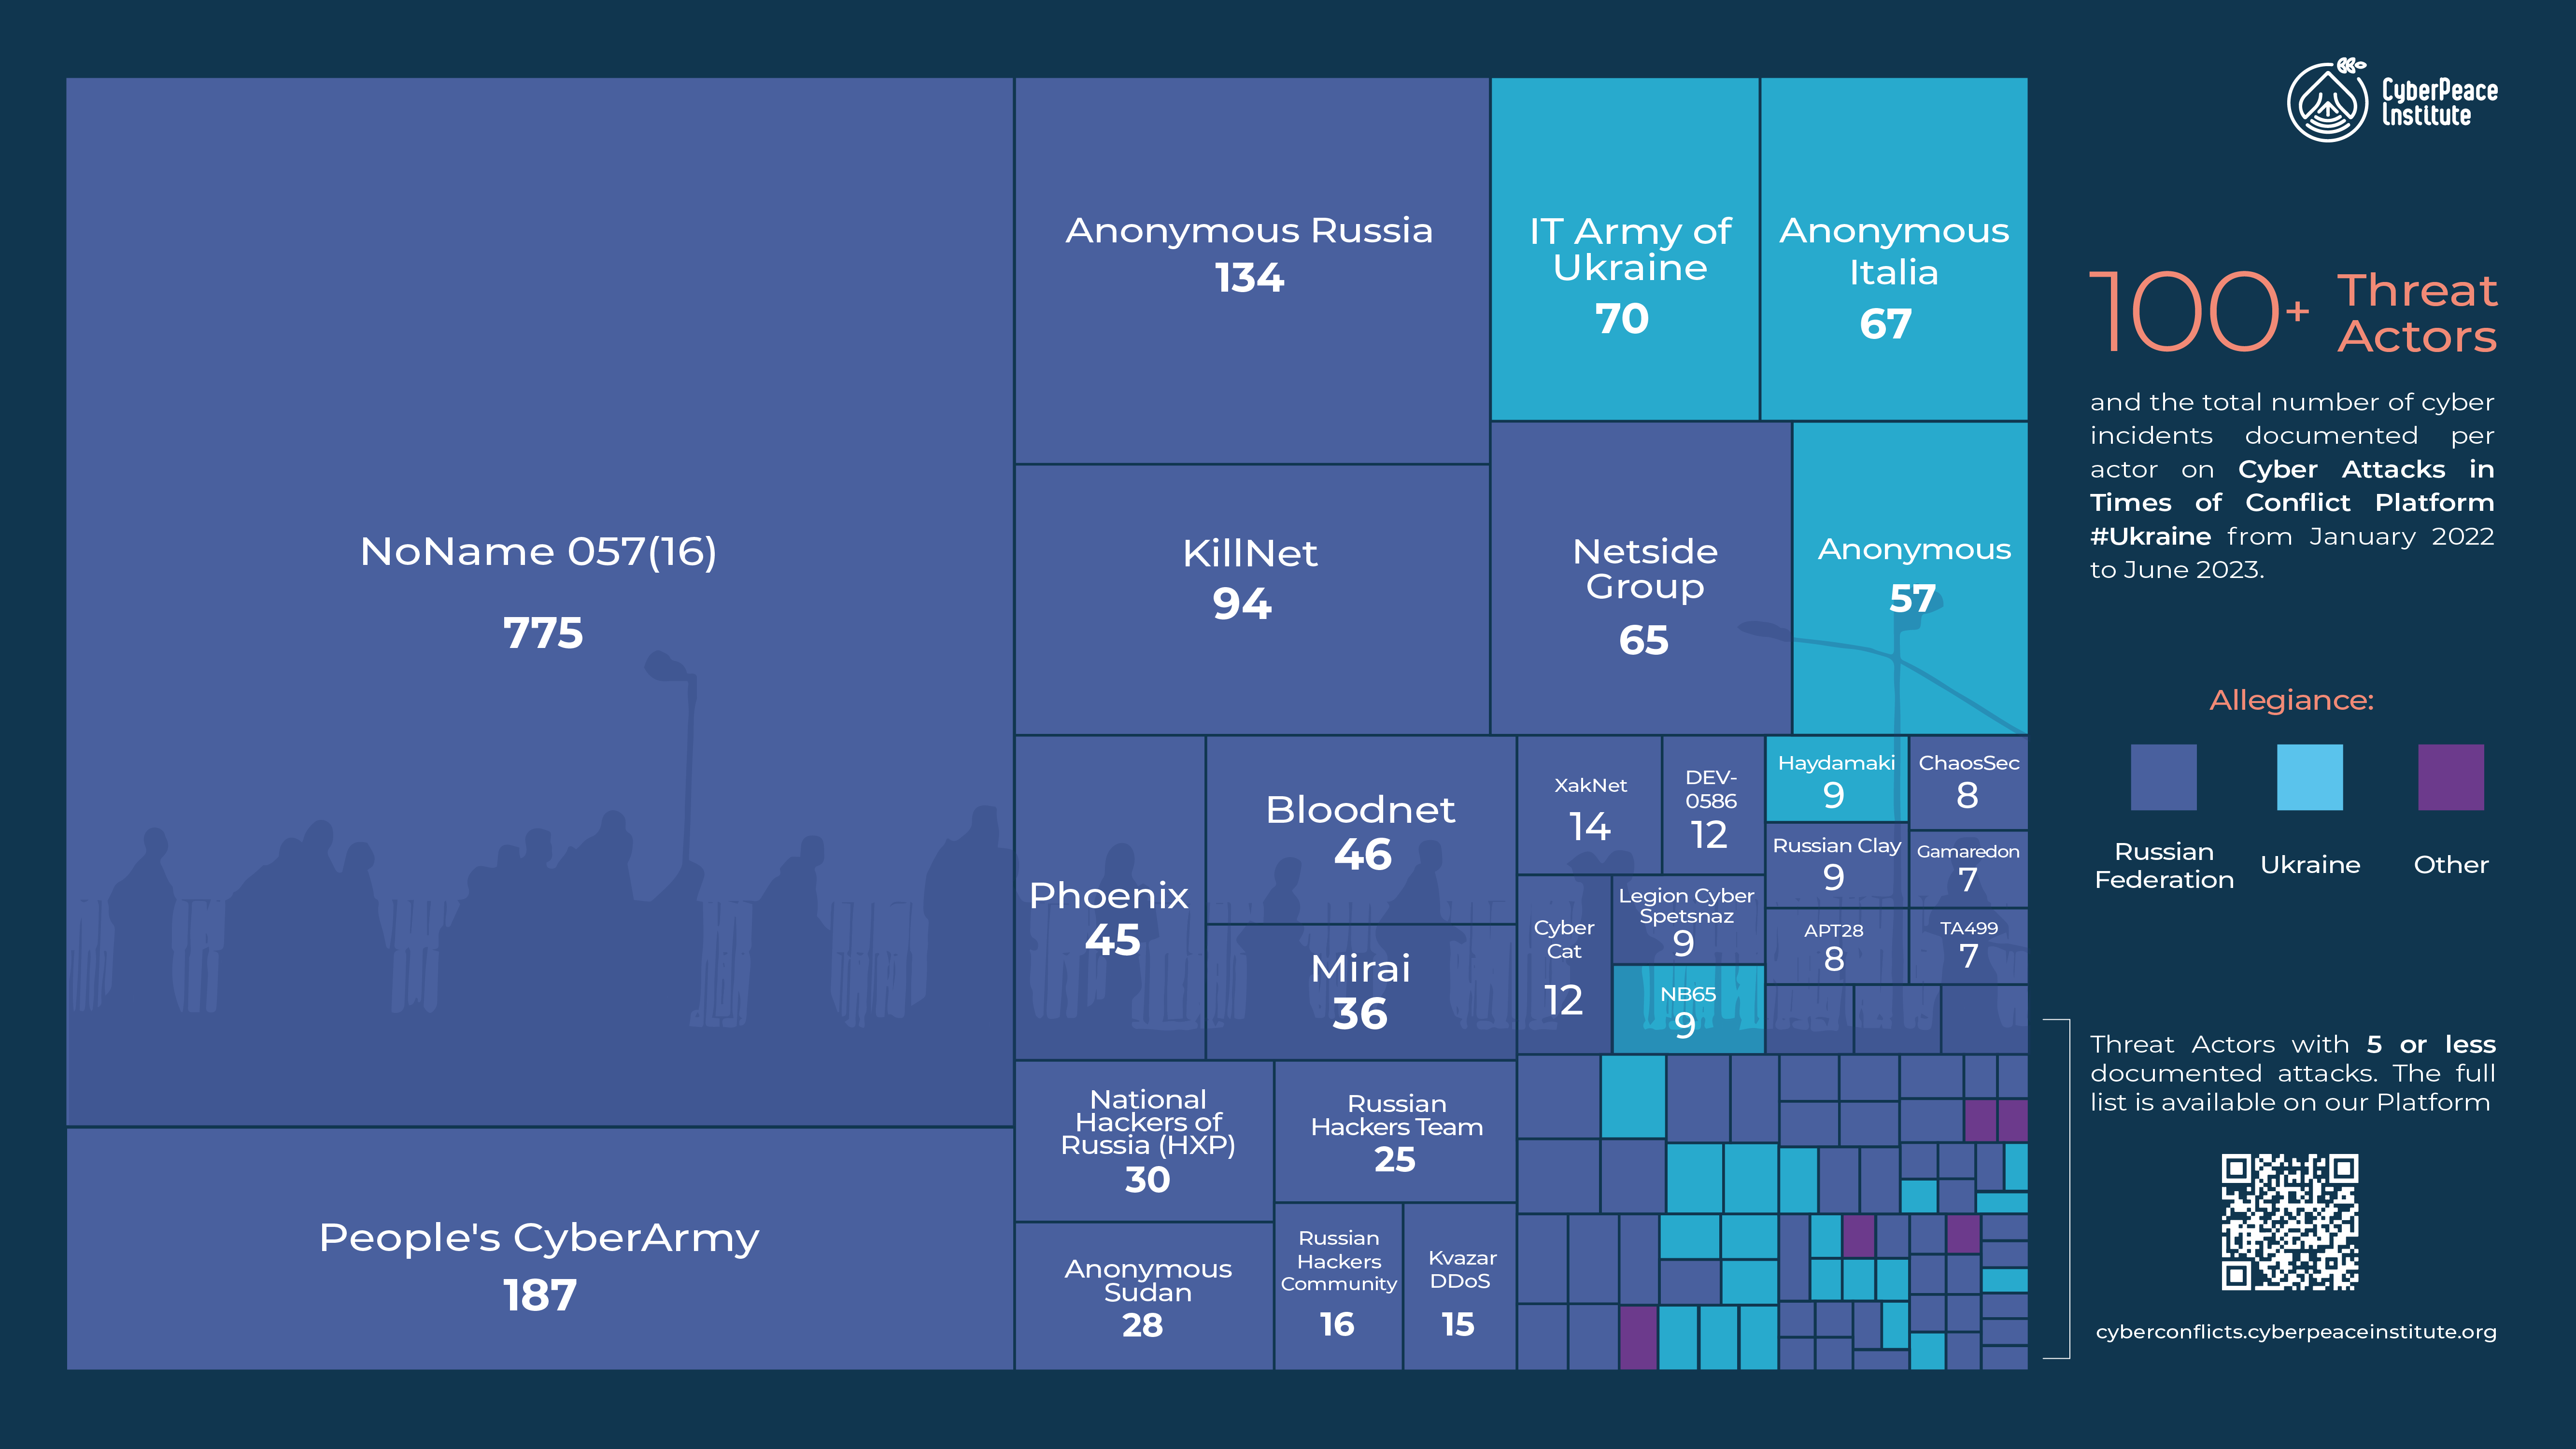
\includegraphics[width=1\textwidth]{Images/actors.png}
\caption{\textit{Threat actors overview after Russian Invasion of Ukraine by \textcite{cyberpeaceinstitute_2023_cyber}}}
\label{actors.png}
\end{figure}


\section{Conclusion: Russian Cyber Operations Attempt and Lessons to Learn}

Russian cyber operations during wartime were a practical example of using cyber capabilities within kinetic counterparts. Even some attempt were successful (such as the Viasat and power grid attacks), the cyber-kinetic integration, in this case study, shows as a relatively early-stage and far to be applied with structured doctrines. However, both cyber and military groups were unprepared to sustain long-term conflict. As Wilde stated:

\textit{Russian war-planning has long been underpinned by the assumption that it would be “the militarily inferior party in a regional or large-scale war against a technologically superior adversary.”  This tendency, along with overly secretive and poorly informed preinvasion planning, appears to have been in effect as Moscow (and the West) overestimated its own abilities and underestimated Ukraine, precisely during the period that its own doctrines are considered the most pivotal for information warfare \autocite{wilde_2022_cyber}}

The Russian VIO could not be compared to the United States Cyber Command, which has demonstrated its capabilities during cyber operations against ISIS. In contrast to their American counterparts, Russians are missing central Command \& and Control, which could fill the structural problem that Russian cyber troops are affected by. Furthermore, the fragmentation of cyber fires does not help Russians. Some several cyber vigilantes and hacktivists sometimes conflict with each other \autocite{cyberpeaceinstitute_2023_cyber}. Russia lost the information war, both internally and internationally, while cyber operations were far from strategic assets. Hence, several scholars have stated that this war has shown that cyberspace is not yet a strategic domain. However, this war demonstrated that Russia’s cyber capabilities are not best suited for a military scenario differently from peacetime, while simultaneously confirming at the same time the problematic coercive issue of cyber operations. Studying the application of cyber operations during contemporary war scenarios is invaluable for acquiring knowledge, and the ongoing conflict between Russia and Ukraine is a crucial milestone in the development of the cyber field.

 
This case study allowed us to gain important insights and lessons learned regarding cyber capabilities during war. To link the key characteristics of cyber capabilities and capacities to the power’s projection, we will use the framework developed by \textcite{vanhaaster_2016_assessing}. The framework helps us to distinguish the political, informational, economic and military dimensions of them. 

\begin{table}[h]
    \centering
    \caption{State’s Power Instruments and Cyber Capacities}
    \label{tab:power-instruments}
    \begin{tabular}{|c|p{8cm}|}
        \hline
        Power Instrument & Capabilities \\
        \hline
        \textbf{Political} & 
        \begin{itemize}
            \item Deterrence
            \item Political Alliances
            \item Involvement of Private Sector
            \item Awareness campaign aimed at SMEs and Public Administrations
        \end{itemize} \\
        \hline
        \textbf{Informational} &  
        \begin{itemize}
        \item Intelligence gathering
        \end{itemize} \\
        \hline
        \textbf{Economical} & 
        \begin{itemize}
            \item Protect Critical Infrastructure
            \item Invest in Skills and Infrastructure
        \end{itemize} \\
        \hline
        \textbf{Military} & 
        \begin{itemize}
            \item Integration of Cyber-Kinetic (C\&C)
            \item Use of Preventive (Offensive) Attacks
        \end{itemize} \\
        \hline
    \end{tabular}
\end{table}



\textbf{Political}

The deterrence has changed its form since the nuclear confrontation during the Cold War. Making the attack more costly than the defence is one of the key features of deterrence in cyberspace, understood as deterrence by denial \autocite{nye_2017_deterrence}. As we analysed in the chapter, cyber operations to physically destroy critical infrastructure were less relevant instead of operations to disrupt or gather intelligence. Firstly, the destructive cyber-attacks are more expensive than the defence framework to counterattack it. For instance, the Stuxnet operation cost \$300 million against \$14 million for the defence \autocite{slayton_2017_what}. The Stuxnet operation, however, was only the first successful offensive operation of this type, which required years of preparation. This type of operation during wartime is less important from the operational perspective due to the planning and the scope. Why a country at war should use a million-dollar cyberattack to disrupt a critical infrastructure when it could use kinetic weapons? The Viasat hack was indeed necessary to disrupt the satellite military communication and to surprise the military counterpart with a full-scale offensive. However, for how much it was well executed, Ukraine (and its allies) has rapidly minimized the issues with other satellite providers (such as Starlink). 

This cyber realm of this war also represents something old in the history of conflict. Alliances can change the course of the war. The support of the Western countries was and is at the time of writing one of the main reasons for the resistance of Ukraine. The value of the cooperation since the Crimea annexation in 2014 has continuously increased. Ukraine's cyber policy has been revolutionised and conforms to NATO standards, abandoning the Soviet style of information war. Moreover, the alliance does not only benefit one part, but the Ukrainian experience was a big value for shaping NATO tactics even in cyberspace. 

Incorporating the private sector into national cyber policies, even during wartime, serves as another significant factor contributing to Ukraine's resilience. The role of big tech companies and their experience in the cyber field have been recognised by scholars. Notably, the disparity between national cyber capabilities and those possessed by the private sector in areas such as cyber threat intelligence and cloud services is evident. This experience presents a dilemma regarding the outsourcing of certain cyber defensive tasks to the private sector.

The increasing collaboration between the private sector in cyberspace and the government presents a unique dynamic, It has been acknowledged that these alliances frequently have cyber capabilities that are equal to or even better than those of state actors. This underscores the ongoing process of de-sovereignisation of defence, attributed in part to the forces of globalization. As a result, this evolution tests conventional national defence borders and highlights the importance of public-private partnerships in enhancing a country's cyber resilience.

A thorough awareness campaign aimed at SMEs and Public Administration should be a political priority to improve their capacity to fend off interruptions, even relatively manageable DDoS attacks. Due to their distinctive nature, hacktivists' actions have attracted a lot of attention during this battle. These cyber actors have maintained a high profile by publicly claiming responsibility for their attacks and openly identifying their victims. Notably, there have been instances where the websites of SMEs and public entities fell victim to prolonged, consecutive cyberattacks. The awareness campaign is designed to prompt proactive thinking within the management of these organizations. It serves as a response to warnings of potential targeting and aims to equip them with the knowledge and resources necessary to prevent or mitigate cyber threats effectively.

\textbf{Informational}

Intelligence gathering during wartime is the cornerstone not only for cyber operations but also for kinetic ones. During pre-war, intelligence served to shape the operational and tactical level avoiding that troops navigate in the shadows. The main reason for the Russian failure is often associated with an intelligence failure, since 3-day military operations were expected, with the Ukrainian army laying down their weapons. Russia has few times attacked Ukraine with kinetic weapons on the logistic sites where Western types of equipment were delivered, underlying the difficulties in gathering information. On the other side, Ukrainians with open source intelligence techniques have discovered the location of Russians who were using social media to post videos and photos on the frontline and while using dating app \footnote{A recent case study was analysed here: https://www.huckmag.com/article/how-tinder-became-a-weapon-in-the-russia-ukraine-war}.

\textbf{Economical}

Since 2014, Ukraine has been repeatedly targeted with cyberattacks on its critical infrastructure, including power grids, transportation networks, and financial systems. While some of these attacks were unsuccessful, the \textit{NotPetya} attack, in particular, caused significant disruptions to Ukraine's energy infrastructure. The ramifications of such cyber incidents serve as a stark reminder of the need for substantial investment in safeguarding critical infrastructure. This imperative is not a mere rhetorical expression; it's a pragmatic policy aimed at nurturing a skilled workforce to enhance cyber resilience. Whether one is involved in offensive or defensive cyber operations, the core skill sets required remain the same. The creation of highly specialised units dedicated to countering cyber threats is a key determinant of success in this domain, as well as training and educational programs with these specific aims. In a human-crafted environment, it is the human factor that can make all the difference.

\textbf{Military}

This conflict has shown that we are far from strategic use of cyber operations due to their lack of integration with kinetic weapons and strategies. A unified Command \& Control for both kinetic and cyber operations was not present for both countries involved, as well a few offensive capabilities were deployed. In the Ukraine-Russia War, cyberspace was less used in a militarised manner, for what was possible to see from open sources. The failure of the integration of both instruments lies down to the organisational issues, lack of training and workforce and military/political will.  Cyber operations have been difficult to incorporate into the normal defence planning process, which is usually focused on a single theatre and allotting troops and weapons by phases of conflict. Cyber operations struggle with assured access, good estimates of effectiveness or extent of damage, or even certainty about how long they will work \autocite{lonergan_2021_cyber}. As \textcite{baetman_2022_russias} stated, the effectiveness of integrated cyber-kinetic fires depends on the level of coordination between cyber and kinetic operations. In some cases, cyber and kinetic fires may achieve unity of purpose through loose alignment or close coordination, while in other cases, their effects may be less cumulative or even unintended. The accumulated experience with cyber weapons has not yet achieved the same maturity as that with kinetic weapons \autocite{dykstra_2020_differentiating}. 



